\documentclass[10pt]{article}
\usepackage[margin=1in]{geometry}
\usepackage[T1]{fontenc}
\usepackage{mathptmx}
\usepackage[scaled=0.9]{helvet}
\usepackage{microtype}
\usepackage{amsmath,amssymb}
\usepackage{graphicx}
\usepackage{booktabs}
\usepackage{multirow}
\usepackage{xcolor}
\usepackage{caption}
\usepackage{subcaption}
\usepackage{enumitem}
\usepackage{tikz}
\usetikzlibrary{positioning,fit,arrows.meta,backgrounds,calc}
\usepackage[numbers,sort&compress]{natbib}
\usepackage[colorlinks=true,linkcolor=blue!50!black,citecolor=blue!50!black,urlcolor=blue!50!black]{hyperref}

\captionsetup{font=small,labelfont=bf}
\setlist{nosep,leftmargin=*}
\newcommand{\ie}{i.e.,\ }
\newcommand{\eg}{e.g.,\ }
\newcommand{\pairs}[2]{#1/#2}

\title{\textbf{BarLine Dance: Bar-Level Planning and Seam Completion\\for Music-Driven Choreography from In-the-Wild Videos}}
\author{Pei Yu}
\date{}

\begin{document}
\maketitle

\begin{abstract}
Music-driven dance generation is judged, above all, by whether the dancer moves \emph{with} the song: poses should arrive on the beat, steps should land in time, and the energy of the dance should rise and fall with the music.
End-to-end generators that model dance as one continuous signal tend to produce plausible poses whose timing is only loosely tied to the particular song, while compositional methods that plan a sequence of reusable movements leave open the question of \emph{when}, inside each unit, the movement happens.
We present \textbf{BarLine Dance}, a planner--completion system that uses the musical \emph{bar} as its unit of choreography.
A discrete-diffusion planner assigns one movement class to every bar of a song; a label-to-motion stage retrieves real bar-length recordings of that class and chooses among them with music-aware criteria---a learned seam selector, same-dancer phrase continuation, a step-lock filter that places foot landings just after the song's beats, and an energy-following filter that ties movement speed to loudness; a diffusion model then redraws only the few frames around each bar line.
The movement library is built from in-the-wild dance videos through content-aware clip cutting and world-grounded 3D human recovery.
Because standard scalar metrics repeatedly failed to reflect what viewers see, we evaluate with metrics that each carry an explicit null control, report per-clip paired sign tests, and treat rendered video as the final arbiter.
On a held-out split of an in-the-wild corpus, the step-lock variant raises the lock of foot landings to the song's beat from $0.094$ to $0.224$ (ground truth $0.155$; the same ground truth scored against another song's grid reads $0.016$), and the energy-following variant raises the correlation between loudness and on-screen movement speed from $-0.021$ to $+0.333$ on eight full songs.
We also document where our own metrics were saturated or gameable, and the limits of a single-creator corpus.
\end{abstract}

% =====================================================================
\section{Introduction}
\label{sec:intro}

Dancing to music is a problem of timing as much as of movement.
A viewer forgives a dancer for choosing a simple step, but not for arriving late: in good choreography each beat is the \emph{end point} of a pose, steps land in time, and quiet passages feel different from the chorus.
Learning this from data is hard for two reasons.
First, high-quality 3D dance capture is scarce and expensive; the widely used AIST++ corpus~\cite{li2021aist} and FineDance~\cite{li2023finedance} cover a limited set of dancers, genres and songs.
Second, timing is a fine-grained, song-specific property that most training objectives do not isolate: a model can match the distribution of poses, and even the global beat statistics, while its accents fall at positions unrelated to the song it is dancing to.

Music-to-dance research has explored two broad families of methods.
\emph{End-to-end generators}---autoregressive models~\cite{lee2019dancing,huang2021dancerevolution,li2021aist}, VQ-VAE with actor--critic GPT~\cite{siyao2022bailando} and diffusion models~\cite{tseng2023edge,li2024lodge}---map audio features directly to motion.
They produce smooth, varied motion but offer little explicit structure, and long sequences tend to drift.
\emph{Compositional methods} instead treat choreography as a sequence of reusable units: motion graphs~\cite{kovar2002motiongraphs} and ChoreoMaster~\cite{chen2021choreomaster} stitch captured segments, Lodge~\cite{li2024lodge} generates characteristic dance primitives as a coarse plan, and the atomic-movement framework of Cai et al.~\cite{cai2026atomic} plans a sequence of interpretable atomic movements with a full-music-aware planner and then synthesizes the motion with a transition-aware diffusion model that retrieves movement prototypes.
Planning at the unit level gives structure and editability, but it moves the timing problem \emph{inside} the unit: once the planner decides \emph{what} to dance in a span and the span boundaries sit on the beat grid, a retrieved prototype is typically stretched uniformly to fill the span, so its accents land wherever the stretching puts them (Fig.~\ref{fig:schematic}a).
Change the song and the accents stay at the same relative positions.

We found this to be the dominant defect of a planner--completion system trained on in-the-wild data.
Diagnostic measurements pointed consistently in one direction (Sec.~\ref{sec:ablation}): aggregate pose statistics already matched ground truth, retrieval was not the bottleneck, and the completion model reduced rather than caused the timing loss---yet the generated dances did not lock to the beat grid of their own song, whereas real dances do.
No stage below the planner decided \emph{when} a movement happens within its unit.

\textbf{BarLine Dance} addresses this by making the musical bar the unit of choreography and moving the timing decision into the label-to-motion stage, where real recordings of the chosen class compete on how well their own timing fits \emph{this} song.
Our contributions are:
\begin{itemize}
  \item \textbf{A bar-level planner--completion pipeline trained on in-the-wild video.} Songs are cut on a 4-beat bar grid, a discrete-diffusion planner emits one token per bar, and a seam-only diffusion completion keeps the retrieved motion intact away from bar lines (Sec.~\ref{sec:method}).
  \item \textbf{Music-aware label-to-motion.} Among the real recordings that match a bar's label, candidates are selected by a learned seam selector, same-dancer phrase continuation, a \emph{step-lock} filter that scores where a candidate's foot landings fall on the song's beat grid, and an \emph{energy-following} filter that matches movement speed to the song's loudness contour. All criteria read only the music and the library, never the target's motion.
  \item \textbf{A corpus pipeline from in-the-wild video to a bar-level movement library}, with content-aware clip cutting, world-grounded 3D recovery~\cite{shen2024gvhmr} and a music-aligned movement vocabulary (Sec.~\ref{sec:corpus}).
  \item \textbf{An evaluation protocol built around controls and video.} Every metric used for a verdict carries a null control (\eg the same ground truth scored against another song's beat grid), comparisons are per-clip paired with sign tests, and rendered videos are reviewed side by side. We report where metrics saturated or were gamed by a variant (Sec.~\ref{sec:experiments}).
\end{itemize}

\begin{figure}[t]
  \centering
  \resizebox{0.86\linewidth}{!}{% Why timing inside the bar matters: uniform stretch vs. music-aware candidate choice.
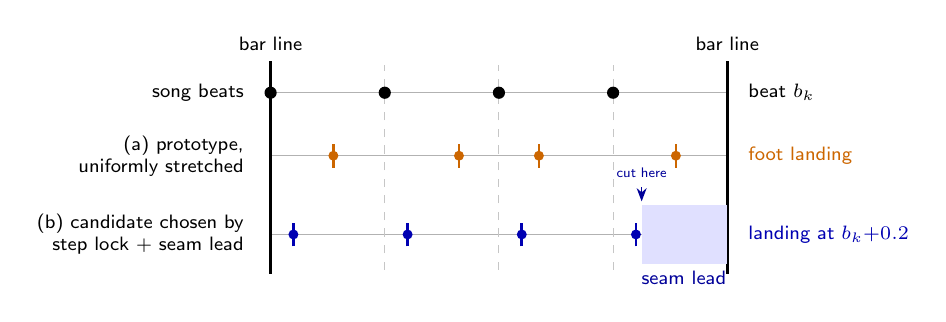
\begin{tikzpicture}[font=\sffamily\scriptsize, x=1.45cm, y=1cm, >=Stealth]
  \def\barlen{4}
  % ---- row labels
  \node[anchor=east, align=right] at (-0.15, 2.0) {song beats};
  \node[anchor=east, align=right] at (-0.15, 1.2) {(a) prototype,\\uniformly stretched};
  \node[anchor=east, align=right] at (-0.15, 0.2) {(b) candidate chosen by\\step lock + seam lead};
  % ---- bar frame
  \foreach \row/\y in {s/2.0, a/1.2, b/0.2} {
    \draw[gray!60] (0,\y) -- (\barlen,\y);
  }
  \foreach \k in {0,1,2,3,4} {
    \draw[gray!45, dashed] (\k, -0.25) -- (\k, 2.35);
  }
  \draw[line width=1.2pt] (0,-0.3) -- (0,2.4) node[above] {bar line};
  \draw[line width=1.2pt] (4,-0.3) -- (4,2.4) node[above] {bar line};
  % beats (onsets); the song's beat grid is uneven in phase within the bar
  \foreach \k in {0,1,2,3} {
    \fill[black] (\k,2.0) circle (2.2pt);
  }
  \node[anchor=west] at (4.1,2.0) {beat $b_k$};
  % ---- (a) uniform stretch: accents land where stretching puts them
  \foreach \t in {0.55, 1.65, 2.35, 3.55} {
    \draw[orange!80!black, line width=1pt] (\t,1.05) -- (\t,1.35);
    \fill[orange!80!black] (\t,1.2) circle (1.8pt);
  }
  \node[anchor=west, text=orange!80!black] at (4.1,1.2) {foot landing};
  % ---- (b) landings 0.2 beat after the beat
  \foreach \k in {0,1,2,3} {
    \pgfmathsetmacro\t{\k+0.2}
    \draw[blue!70!black, line width=1pt] (\t,0.05) -- (\t,0.35);
    \fill[blue!70!black] (\t,0.2) circle (1.8pt);
  }
  \node[anchor=west, text=blue!70!black] at (4.1,0.2) {landing at $b_k{+}0.2$};
  % seam lead: cut 0.75 beat before the next bar line
  \fill[blue!12] (3.25,-0.18) rectangle (4,0.58);
  \node[text=blue!60!black] at (3.62,-0.35) {seam lead};
  \draw[<-, blue!60!black] (3.25,0.62) -- ++(0,0.18) node[above, font=\sffamily\tiny]{cut here};
\end{tikzpicture}
}
  \caption{\textbf{Timing inside a bar.} The planner fixes \emph{what} is danced in a bar and the beat grid fixes the bar lines. (a) Uniformly stretching a prototype to fill the bar puts its foot landings wherever the stretch puts them, unrelated to this song's beats. (b) BarLine Dance instead chooses, among real recordings of the planned class, the ones whose landings fall shortly after the song's beats ($0.2$ beat, measured on training data), and cuts each unit $0.75$ beat before the next bar line so that every downbeat is a single dancer's approach and arrival.}
  \label{fig:schematic}
\end{figure}

% =====================================================================
\section{Related Work}
\label{sec:related}

\paragraph{Music-to-dance generation.}
Early learning-based systems decomposed dance into units and learned to compose them~\cite{lee2019dancing}, or generated long sequences with curriculum-trained sequence models~\cite{huang2021dancerevolution}.
AIST++ and the FACT transformer~\cite{li2021aist} established a common benchmark with FID-style and beat-alignment metrics.
Bailando~\cite{siyao2022bailando} quantizes poses into a choreographic memory and composes them with an actor--critic GPT.
EDGE~\cite{tseng2023edge} introduced a transformer diffusion model conditioned on Jukebox features~\cite{dhariwal2020jukebox,castellon2021jukemir} with editing through inpainting; our completion model follows its denoiser design.
Lodge~\cite{li2024lodge} generates long dances coarse-to-fine through characteristic dance primitives, and FineDance~\cite{li2023finedance} contributes finer-grained genres and hand motion.
Our work differs in its data source (in-the-wild video rather than motion capture) and in placing the timing decision in a retrieval stage conditioned on the song.

\paragraph{Compositional and retrieval-based choreography.}
Motion graphs~\cite{kovar2002motiongraphs} synthesize new motion by traversing transitions between captured clips; ChoreoMaster~\cite{chen2021choreomaster} builds a choreography-oriented graph over music and dance units with learned embeddings.
Cai et al.~\cite{cai2026atomic} represent choreography as a sequence of discovered atomic movements, predict their type, timing and duration with a full-music-aware planner, and synthesize motion with a transition-aware diffusion model that retrieves and re-creates movement prototypes.
BarLine Dance follows this planner--completion paradigm and adapts it in three ways: the unit is a musical bar rather than a variable-length segment, the library consists of in-the-wild recordings reconstructed in 3D, and the choice among same-class candidates is driven by music-aware timing and energy criteria rather than by a uniformly stretched prototype.

\paragraph{Diffusion models for motion.}
Denoising diffusion~\cite{ho2020ddpm} has become a standard generator for human motion~\cite{tevet2023mdm,tseng2023edge}.
Discrete diffusion~\cite{austin2021d3pm} extends the framework to categorical sequences, which we use for the bar planner, and diffusion inpainting~\cite{lugmayr2022repaint} lets a model redraw a masked region consistently with its context, which we use to regenerate only the neighbourhood of each bar line.

\paragraph{Human motion from monocular video.}
Parametric body models~\cite{loper2015smpl,pavlakos2019smplx} and 2D pose estimators~\cite{yang2023dwpose,xu2022vitpose} make it possible to recover 3D motion from ordinary video.
World-grounded methods such as WHAM~\cite{shin2024wham} and GVHMR~\cite{shen2024gvhmr}, combined with visual odometry~\cite{teed2023dpvo}, separate the body's global trajectory from camera motion, which is essential for dance where the camera itself often moves.
We rely on GVHMR with DPVO to turn short-form dance videos into a 3D corpus.

\paragraph{Pose-driven character animation.}
Image-to-video diffusion models conditioned on a pose sequence~\cite{hu2024animateanyone,wan2025} can animate a single character image.
We use such a model only for presentation and review: the generated 3D dance is projected to a 2D pose video that drives a character, and the rendered video is part of our evaluation because some defects appear only after projection (Sec.~\ref{sec:results}).

% =====================================================================
\section{Method}
\label{sec:method}

Figure~\ref{fig:arch} gives an overview.
Offline, in-the-wild videos are turned into a library of bar-length 3D movements with a movement vocabulary (Sec.~\ref{sec:corpus}).
At inference, given only a song, the planner assigns a class to every bar (Sec.~\ref{sec:planner}), the label-to-motion stage fills each bar with a real recording chosen by music-aware criteria (Sec.~\ref{sec:retrieval}), and a seam completion model smooths the bar lines (Sec.~\ref{sec:completion}).

\begin{figure}[t]
  \centering
  \resizebox{\linewidth}{!}{% Overall architecture of BarLine Dance (TikZ).
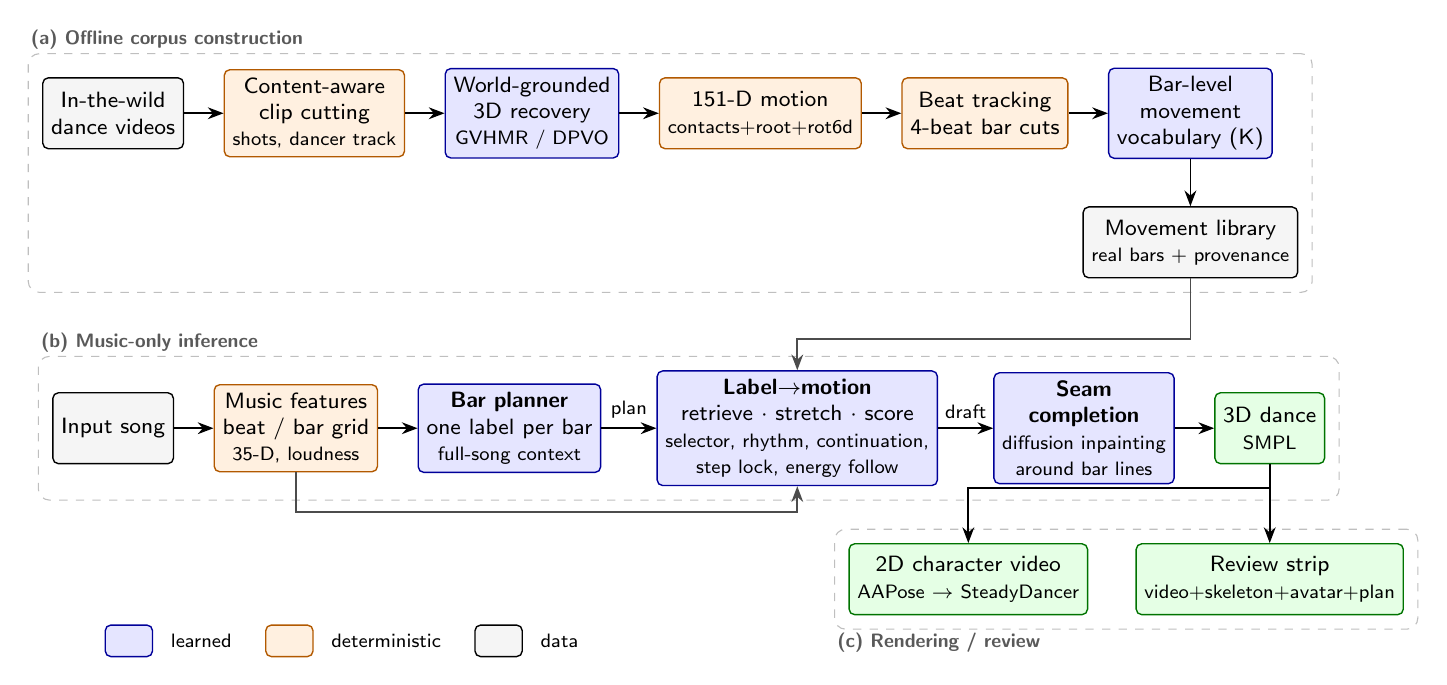
\begin{tikzpicture}[
  font=\sffamily\footnotesize,
  >=Stealth,
  box/.style={draw, rounded corners=2pt, align=center, minimum height=9mm, inner sep=3pt, line width=0.5pt},
  data/.style={box, fill=gray!8},
  learn/.style={box, fill=blue!10, draw=blue!60!black},
  rule/.style={box, fill=orange!12, draw=orange!70!black},
  outp/.style={box, fill=green!10, draw=green!45!black},
  arr/.style={->, line width=0.6pt},
  lane/.style={draw=gray!50, dashed, rounded corners=4pt},
  lbl/.style={font=\sffamily\scriptsize\bfseries, text=gray!70!black, anchor=south west, inner sep=1pt}
]
% ---------------- Offline: corpus construction ----------------
\node[data] (vid) at (0,0) {In-the-wild\\dance videos};
\node[rule, right=5mm of vid] (ing) {Content-aware\\clip cutting\\{\scriptsize shots, dancer track}};
\node[learn, right=5mm of ing] (hmr) {World-grounded\\3D recovery\\{\scriptsize GVHMR / DPVO}};
\node[rule, right=5mm of hmr] (rep) {151-D motion\\{\scriptsize contacts+root+rot6d}};
\node[rule, right=5mm of rep] (bar) {Beat tracking\\4-beat bar cuts};
\node[learn, right=5mm of bar] (voc) {Bar-level\\movement\\vocabulary (K)};
\node[data, below=6mm of voc] (lib) {Movement library\\{\scriptsize real bars + provenance}};
\draw[arr] (vid) -- (ing);
\draw[arr] (ing) -- (hmr);
\draw[arr] (hmr) -- (rep);
\draw[arr] (rep) -- (bar);
\draw[arr] (bar) -- (voc);
\draw[arr] (voc) -- (lib);
\begin{scope}[on background layer]
  \node[lane, fit=(vid)(ing)(hmr)(rep)(bar)(voc)(lib), inner sep=5pt, label={[lbl]north west:(a) Offline corpus construction}] (laneA) {};
\end{scope}

% ---------------- Inference ----------------
\node[data] (song) at (0,-4.0) {Input song};
\node[rule, right=5mm of song] (mus) {Music features\\beat / bar grid\\{\scriptsize 35-D, loudness}};
\node[learn, right=5mm of mus] (plan) {\textbf{Bar planner}\\one label per bar\\{\scriptsize full-song context}};
\node[learn, right=7mm of plan, minimum width=33mm] (ret) {\textbf{Label$\rightarrow$motion}\\retrieve $\cdot$ stretch $\cdot$ score\\{\scriptsize selector, rhythm, continuation,}\\{\scriptsize step lock, energy follow}};
\node[learn, right=7mm of ret] (comp) {\textbf{Seam}\\\textbf{completion}\\{\scriptsize diffusion inpainting}\\{\scriptsize around bar lines}};
\node[outp, right=5mm of comp] (d3) {3D dance\\{\scriptsize SMPL}};
\draw[arr] (song) -- (mus);
\draw[arr] (mus) -- (plan);
\draw[arr] (plan) -- node[above, font=\sffamily\scriptsize]{plan} (ret);
\draw[arr] (ret) -- node[above, font=\sffamily\scriptsize]{draft} (comp);
\draw[arr] (comp) -- (d3);
\draw[arr, draw=gray!60!black] (lib.south) |- ([yshift=4mm]ret.north) -- (ret.north);
\draw[arr, draw=gray!60!black] (mus.south) -- ++(0,-5mm) -| (ret.south);
\begin{scope}[on background layer]
  \node[lane, fit=(song)(mus)(plan)(ret)(comp)(d3), inner sep=5pt, label={[lbl]north west:(b) Music-only inference}] (laneB) {};
\end{scope}

% ---------------- Rendering ----------------
\node[outp, below=10mm of d3] (strip) {Review strip\\{\scriptsize video+skeleton+avatar+plan}};
\node[outp, left=6mm of strip] (r2d) {2D character video\\{\scriptsize AAPose $\rightarrow$ SteadyDancer}};
\draw[arr] (d3) -- (strip);
\draw[arr] (d3.south) |- ++(-5mm,-3mm) -| (r2d.north);
\begin{scope}[on background layer]
  \node[lane, fit=(strip)(r2d), inner sep=5pt, label={[lbl, anchor=north west]south west:(c) Rendering / review}] {};
\end{scope}

% legend
\node[learn, minimum height=4mm, minimum width=6mm, inner sep=1pt] (lg1) at (0.2,-6.7) {};
\node[right=1mm of lg1, font=\sffamily\scriptsize] (t1) {learned};
\node[rule, minimum height=4mm, minimum width=6mm, inner sep=1pt, right=3mm of t1] (lg2) {};
\node[right=1mm of lg2, font=\sffamily\scriptsize] (t2) {deterministic};
\node[data, minimum height=4mm, minimum width=6mm, inner sep=1pt, right=3mm of t2] (lg3) {};
\node[right=1mm of lg3, font=\sffamily\scriptsize] {data};
\end{tikzpicture}
}
  \caption{\textbf{BarLine Dance overview.} (a) Offline, in-the-wild dance videos are cut into clips, reconstructed in world coordinates, converted to a 151-D motion representation, cut into 4-beat bars on the music's beat grid and grouped into a bar-level movement vocabulary; the bars form a retrieval library with provenance. (b) At inference the system reads only the song: a bar planner emits one label per bar, the label-to-motion stage retrieves, time-stretches and scores same-class candidates from the library, and a diffusion model redraws the neighbourhood of each bar line. (c) The 3D result is reviewed as a side-by-side strip and rendered as a 2D character video.}
  \label{fig:arch}
\end{figure}

\subsection{From in-the-wild video to a bar-level library}
\label{sec:corpus}

\paragraph{Content-aware clipping.}
Short-form dance uploads contain shot changes, intros without a dancer and occasional group scenes.
Instead of cutting at fixed durations, we run a single detection pass over each upload and cut at shot changes and at stretches where no dancer is on screen; the dancer is followed as a track with DWPose~\cite{yang2023dwpose}, and the maximum clip length is measured rather than assumed, since it trades segmentation granularity against monocular drift.

\paragraph{World-grounded 3D recovery.}
Each clip is reconstructed with GVHMR~\cite{shen2024gvhmr} using DPVO~\cite{teed2023dpvo} for camera motion, giving SMPL-X~\cite{pavlakos2019smplx} body parameters in a gravity-aligned world frame.
DPVO's frequent divergence on our clips turned out to be caused by reduced-precision (TF32) matrix arithmetic; disabling it made all 18 previously diverging test clips converge.
The SMPL-X body is mapped to 24 SMPL~\cite{loper2015smpl} joints (the two hand joints are set to identity and flagged) and converted to a 151-D representation at 30\,fps: 4 foot-contact channels, 3 root translations, and 24 joint rotations in the 6-D representation~\cite{zhou2019rot6d}, in a z-up world frame.

\paragraph{Bars and vocabulary.}
Music is represented by 35-D per-frame features computed with librosa~\cite{mcfee2015librosa} (onset envelope, 20 MFCCs, 12 chroma, onset peaks and a beat indicator).
We track beats~\cite{ellis2007beat} and cut every clip into 4-beat bars, so that a movement unit is exactly one bar (median $2.00$\,s, maximum $2.97$\,s in our corpus).
Movement classes are obtained in two steps.
A discovery vocabulary of 20 classes is formed by clustering bar embeddings.
Because that vocabulary turned out to be poorly predictable from music---its labels were read from bar music below the majority-class floor---the planner and library use a second, \emph{music-aligned} vocabulary: a canonical correlation analysis between sub-bar music features and an 11-number motion descriptor, followed by $k$-means with $k{=}8$, fit on training bars only.
Every library bar keeps its provenance (upload, clip, dancer track), which later stages use for continuation and for excluding the query's own performance from retrieval.

\subsection{Bar planner}
\label{sec:planner}

The planner predicts a sequence of labels $y_{1:K}$, one per bar, from the bar-pooled music features $m_{1:K}$ of the whole song.
It is a transformer encoder trained as a discrete diffusion model~\cite{austin2021d3pm} with a uniform transition kernel and $x_0$ parameterization; music enters through per-channel normalization stored with the checkpoint, and classifier-free guidance is enabled by dropping the music condition during training.
Using one token per bar was motivated by a measurement on an earlier frame-level planner: adjacent frames share a label 98.8\% of the time, so each real decision was worth about 1\% of the training loss, and the planner changed label from one bar to the next only 58.3\% of the time against 78.4\% in ground truth.
Plans are sampled stochastically and can be pinned for controlled comparisons.

\subsection{Label-to-motion: choosing real recordings with the song}
\label{sec:retrieval}

For each bar $k$ with label $y_k$, candidates are library bars of the same class whose duration lies within a band around the target, excluding every recording of the query performance.
Each candidate is time-stretched to the bar.
The core idea of BarLine Dance is that the \emph{choice among these candidates} is where timing is decided.
The criteria below are applied as successive keep-fractions (each keeps the best fraction of the remaining candidates), followed by temperature sampling.

\paragraph{Seam selector.}
A learned selector scores the join between the previous bar's motion and a candidate: canonicalized pose, velocity and contact across the seam.
We keep the best fraction by seam cost (a \emph{join band}), which avoids visible pops while leaving room for the music criteria.

\paragraph{Phrase continuation and seam lead.}
Cutting between dancers at every bar line produces reversals right after the line.
When the dancer of the previous bar has a next bar in the library, we let that recording continue (for up to four bars within a phrase, without replaying the same material), so that most bar lines stop being a cut.
In addition, each unit is cut $0.75$ beat \emph{before} the next bar line (the \emph{seam lead}), so that the downbeat itself is one real dancer's approach and arrival rather than a splice.

\paragraph{Step lock.}
For each candidate we locate its source foot landings (world foot speed dropping from above $0.6$ to below $0.25$\,m/s), map them through the time-stretch into the target bar, and score them on the song's beat grid as $\frac{1}{L}\sum_{\ell}\cos\!\big(2\pi(\phi_\ell - \delta)\big)$, where $\phi_\ell$ is the landing's beat phase and $\delta{=}0.2$ beat is the landing lag of real dancers measured on the training split.
The step-lock filter keeps the fraction of candidates with the highest score, evaluated over a whole phrase at phrase starts.
The score a candidate is predicted to achieve correlates with the lock it realizes in the output (Spearman $+0.63$).

\paragraph{Energy following.}
Bar loudness (MFCC $c_0$) is smoothed over neighbouring bars and ranked within the song; its rank is mapped to a target percentile of library movement speed in $[0.15, 0.85]$, and candidates closest to the target speed are kept.
A variant additionally keeps the candidates that come most to rest on the beat as seen by the camera, since timing that is visible in 3D can be lost after projection to the image plane.

\paragraph{Music only.}
Every criterion reads the song (beats, loudness, features) and the library; none reads the target clip's motion.
This is a hard rule in our system: a timing alignment that consulted the ground-truth dance would make the evaluation meaningless.

\subsection{Seam completion}
\label{sec:completion}

The retrieved sequence (the \emph{draft}) is passed to a diffusion model that follows the EDGE denoiser~\cite{tseng2023edge}, conditioned on music and on the draft with a noise mask.
At inference we regenerate only a window of $\pm 8$ frames around each seam (weights reach zero at the window edge, so about 8--10\% of frames are redrawn), in the manner of diffusion inpainting~\cite{lugmayr2022repaint}, and hold the root trajectory to the draft.
This keeps each bar's content a real recording and restricts the generative model to transitions.
A light post-processing step turns the dancer toward the camera, removes planted-foot sliding, and anchors the floor height.

\subsection{Rendering for review}
\label{sec:render}

Two renderings are produced for every result.
A review strip places the source video (for held-out clips), the raw 3D skeleton, a skinned avatar and a timeline of the plan side by side on one stage; the skeleton shows exactly the joints the model produced, and the timeline distinguishes dense splicing from long transition fillers.
A 2D character video is produced by projecting the 3D joints to a 2D pose sequence and driving a pose-conditioned video diffusion model~\cite{wan2025} with a single character image.

% =====================================================================
\section{Experiments}
\label{sec:experiments}

\subsection{Data}
\label{sec:data}

Table~\ref{tab:data} summarizes the corpus.
All clips come from one short-video creator's public uploads; different clips are different performances by the same dancer.
Clips are split by audio-fingerprint connected components so that recordings of the same song fall on the same side.
Most comparisons use the 20 test clips (one per test upload) together with 30 validation clips, and are computed per clip, giving $n{=}50$ paired comparisons.
Full-song results use songs the system dances from start to end.

\begin{table}[t]
  \centering
  \small
  \caption{\textbf{Corpus used in our experiments.} One creator; the split keeps same-song recordings together (see Sec.~\ref{sec:limitations} for the known exceptions).}
  \label{tab:data}
  \begin{tabular}{@{}lr@{}}
    \toprule
    Clips / uploads (total) & 333 / 221 \\
    Train / val / test clips & 278 / 32 / 23 \\
    Train retrieval windows (150 frames, stride 15) & 6{,}112 \\
    Frame rate; motion representation & 30\,fps; 151-D \\
    Music features & 35-D per frame \\
    Bar-length units (4 beats), median / max duration & 2.00\,s / 2.97\,s \\
    Discovery vocabulary / planner vocabulary & 20 / 8 classes \\
    \bottomrule
  \end{tabular}
\end{table}

\subsection{Metrics and protocol}
\label{sec:metrics}

Early in the project, several plausible metrics produced verdicts that the rendered videos contradicted.
We therefore require each metric used for a decision to (i) state what it measures and where it comes from, (ii) separate ground truth from a matched null control, and (iii) be compared per clip against the same baseline with a sign test.
We write \pairs{36}{50} for ``36 of 50 clips move in the stated direction'' and mark $p{<}0.05$ with~$^*$.

\begin{itemize}
  \item \textbf{Foot-landing beat lock.} The step-lock score of Sec.~\ref{sec:retrieval} computed on the output. Control: the same motion scored against another song's beat grid. Ground truth reads $0.155$ against its own song and $0.016$ against another song (\pairs{36}{50}, $p{=}0.003$).
  \item \textbf{Per-beat arrival} (\emph{hit}). At every beat, one minus the ratio of the slowest body speed just around the beat to the fastest speed in a wider window; median over beats. Control: the same readout half a beat off. Ground truth scores higher on-beat than off-beat on \pairs{35}{50} ($p{=}0.007$).
  \item \textbf{Stop-then-burst} (\emph{dipburst}). The rate of abrupt braking followed by a surge near bar lines, used as a veto: a variant that improves arrival by braking artificially is rejected.
  \item \textbf{Loudness following.} Per song, the Spearman correlation between bar loudness and bar mean body speed, and the speed ratio of the loudest to the quietest third of bars. Measured on full songs, in 3D and on the rendered video with ViTPose~\cite{xu2022vitpose}.
  \item \textbf{On/off-beat contrast.} How much more the body comes to rest on beats than half a beat away, measured on the rendered video.
  \item \textbf{Seams and turns.} The fraction of bar lines followed within one beat by a movement reversal, compared with equally smoothed ground truth, and the number of completed turns.
  \item \textbf{Cross-song diversity.} The mean distance between a clip's bars and other clips' bars, which falls when different songs are danced alike.
\end{itemize}

\paragraph{Saturation.}
A metric on which generated variants already beat ground truth cannot rank them.
Our first global beat metric (how much slower the body moves on this song's beats than on another song's) read $0.082$/$0.089$ for ground truth on test/val and between $0.11$ and $0.52$ for every generated variant; we therefore use it only as a veto.
For the same reason, once variants exceeded ground truth on foot-landing lock, we stopped using it to rank further variants.

\subsection{Variants}
Results are reported for the following cumulative variants; each adds switches of Sec.~\ref{sec:retrieval}.
\textbf{A0}: planner, seam selector and seam completion with uniform stretching (the base system).
\textbf{E11}: A0 with gentle motif return and continuity/rhythm keep-fractions.
\textbf{F11}: E11 with seam lead ($0.75$ beat) and in-phrase source continuation without replay.
\textbf{J7}: F11 with step lock (keep 0.3) and a wider join band (0.6).
\textbf{K13}: J7 with energy following (keep 0.3) and camera-plane rest-on-beat selection.
For the seam study we also compare a retrieval-cut baseline with source continuation and a variant that keeps completed turns (no pull back toward the camera).

\subsection{Results}
\label{sec:results}

\paragraph{Steps land on this song's beat.}
Figure~\ref{fig:steplock} shows foot-landing lock on the 50 evaluation clips.
The base system does not lock to the song ($-0.006$).
F11 improves to $0.094$ but stays below ground truth on \pairs{33}{50} clips ($p{=}0.03$); F11 scored against another song's grid reads $-0.001$ (\pairs{35}{50} above it, $p{=}0.007$), so the gain is specific to the song.
With step lock, J2 and J7 reach $0.232$ and $0.224$ (\pairs{37}{48}$^*$ and \pairs{40}{50}$^*$ above F11), exceeding ground truth; the gain replicates on a second, independently sampled plan (J7: $0.200$, \pairs{38}{50}$^*$).
On eight full songs J7 reads $0.163$ against F11's $0.046$ (7/8 songs higher), and $0.016$ against other songs' grids.
Because the filter selects partly on this very quantity, we confirmed the effect on rendered video: J7 comes more to rest on beats than half a beat away on 9/9 songs ($0.609$ vs $0.566$), against 6/9 for F11 and for the source videos.
The operator's verdict after reviewing the renders was that J7 has richer movement and better rhythm control than F11.

\begin{figure}[t]
  \centering
  \begin{subfigure}[t]{0.42\linewidth}
    \centering
    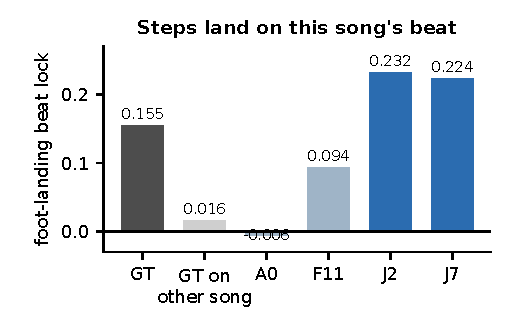
\includegraphics[width=\linewidth]{figures/step_lock.pdf}
    \caption{Foot-landing beat lock (50 clips).}
    \label{fig:steplock}
  \end{subfigure}\hfill
  \begin{subfigure}[t]{0.56\linewidth}
    \centering
    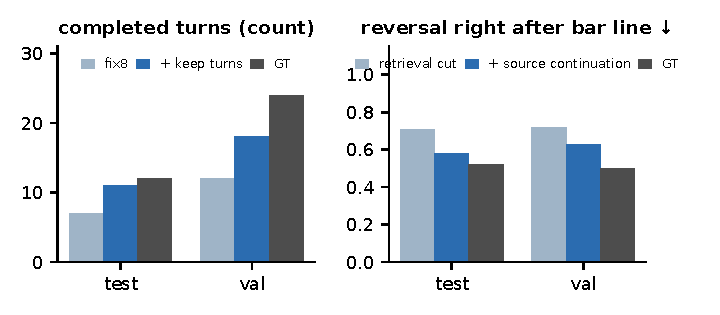
\includegraphics[width=\linewidth]{figures/turns_seams.pdf}
    \caption{Completed turns and reversals after bar lines.}
    \label{fig:seams}
  \end{subfigure}
  \caption{\textbf{Timing and seams.} (a) Ground truth locks to its own song ($0.155$) but not to another song's grid ($0.016$); the base system A0 does not lock at all; step lock (J2, J7) closes and then exceeds the gap. (b) Keeping turns raises completed turns toward ground truth; letting the same dancer continue across bar lines reduces reversals right after the line toward the ground-truth level.}
\end{figure}

\paragraph{Fewer cuts at bar lines, completed turns.}
With retrieval alone, a movement reversal follows $71$--$72\%$ of bar lines within one beat, against $52\%$/$50\%$ in ground truth (test/val).
Source continuation lets the previous bar's dancer continue, so that $73$--$76\%$ of bar lines are no longer cuts, and reversals drop to $58\%$/$63\%$ (Fig.~\ref{fig:seams}).
Removing the slow pull toward the camera, which aborted sustained turns, raises completed turns from $7$ to $11$ on test and from $12$ to $18$ on validation (ground truth $12$ and $24$), and brings the share of off-camera facing from $0.041$/$0.047$ to $0.116$/$0.107$ (ground truth $0.123$/$0.113$).

\paragraph{Following the energy of the song.}
Real dancers speed up in loud passages and slow down in quiet ones; F11 and J7 do not (Fig.~\ref{fig:energy}).
Measured on the rendered 720p videos of eight full songs, K13 raises the correlation between loudness and on-screen speed to $+0.333$ (J7 $-0.021$, F11 $-0.006$; 8/8 songs above J7), the loud-to-quiet speed ratio to $1.192$ (J7 $1.001$; 8/8), and the on/off-beat contrast to $+0.044$ (J7 $+0.028$, F11 $+0.023$; 6/8).
On seven further songs that were not used during development, K13 again follows loudness more closely than J7 ($+0.321$ vs $+0.161$, 6/7) and contrasts on- and off-beat more ($+0.029$ vs $+0.017$, 5/7).
On the short evaluation clips K13 arrives on the beat more often than J7 (\pairs{60}{99}, $p{\approx}0.04$) and less often half a beat off (\pairs{37}{99} higher, $p{\approx}0.01$) while keeping the foot-landing lock; the cost is fewer held poses (\pairs{31}{85} higher, $p{\approx}0.02$).
An earlier energy variant (K5) appeared to keep the beat in 3D but lost it after projection to the image plane: its on/off-beat contrast went from $0.039$ in 3D to $0.026$ on the driving 2D skeleton and $0.019$ on the rendered video, whereas J7 went from $0.044$ to $0.041$ and $0.036$. Energy following had picked faster, more continuous units whose rests happen along the camera's depth axis, so K13 additionally selects on rest-on-beat as seen by the camera.

\begin{figure}[t]
  \centering
  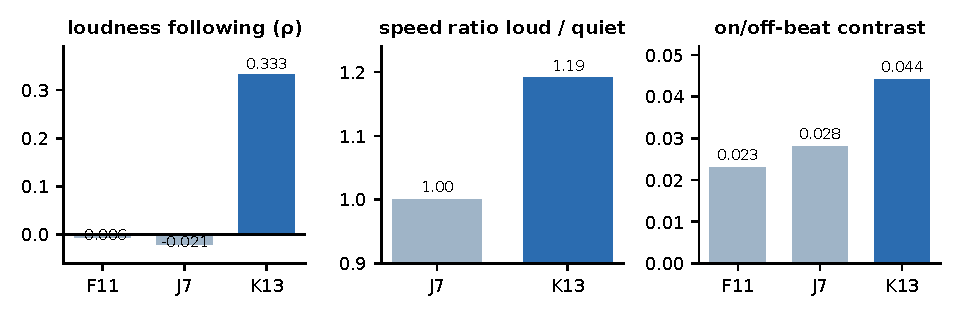
\includegraphics[width=0.88\linewidth]{figures/energy_follow.pdf}
  \caption{\textbf{Following the energy of the song} (eight full songs, measured with ViTPose on the rendered 720p videos). Energy following (K13) makes on-screen movement speed track loudness and increases the contrast between on-beat and off-beat rest. F11 has no recorded loud/quiet ratio on video and is omitted from the middle panel.}
  \label{fig:energy}
\end{figure}

\paragraph{Choreographic statistics.}
Table~\ref{tab:choreo} reports statistics of the base variants on the 50 evaluation clips under one pinned plan.
Seam lead and continuation (F5, the precursor of F11) bring the wrist deceleration before bar lines close to ground truth (preseam $1.037$ vs $1.054$; A0 $1.176$) and increase left--right coordination beyond A0, while motif return (E11) raises bar-level repetition above ground truth ($0.283$ vs $0.189$); F11 removed multi-bar replays (23 $\rightarrow$ 1) and lowered repetition to $0.202$.

\begin{table}[t]
  \centering
  \small
  \caption{\textbf{Choreographic statistics} on 50 clips, one pinned plan. preseam: wrist speed just before the bar line relative to the clip median (ground truth decelerates into the shape); arrive: arrival at bar lines; hold: fraction of held frames; repetition: bar-level self-similarity at 2/4-bar lags; dipburst: stop-then-burst rate (veto). $^*$: $p{<}0.05$ paired against A0.}
  \label{tab:choreo}
  \begin{tabular}{@{}lccccc@{}}
    \toprule
    & preseam & arrive $\uparrow$ & hold & repetition & dipburst $\downarrow$ \\
    \midrule
    Ground truth & 1.054 & 0.637 & 0.072 & 0.189 & 0.099 \\
    \midrule
    A0 & 1.176 & 0.608 & 0.024 & 0.109 & 0.100 \\
    E11 & 1.108 & 0.610 & 0.028 & 0.283 & 0.119 \\
    F5 (seam lead + continuation) & 1.037$^*$ & 0.623 & 0.032 & 0.247 & 0.071 \\
    \bottomrule
  \end{tabular}
\end{table}

\paragraph{A metric that was gamed.}
We also tried to enforce arrival directly by re-generating the middle of each beat interval while keeping the draft at the beats (G series).
On nine whole songs this variant (G17) had the highest per-beat arrival of all variants ($0.651$, above F11 on 7/9 songs), and on the rendered video its arrival came closest to the source videos.
After watching the nine songs side by side, however, the operator judged F11 clearly better than A0, E11 and G17 on rhythm, arrival, variety and transitions.
The explanation was a second metric: G17 produced $2.4\times$ as many stop-then-burst events as F11 ($0.159$ vs $0.067$, higher on 8/9 songs; Fig.~\ref{fig:gaming}).
The arrival metric rewarded artificial braking at every beat.
Since then, arrival is only read together with the stop-then-burst veto and the fraction of held poses.

\begin{figure}[t]
  \centering
  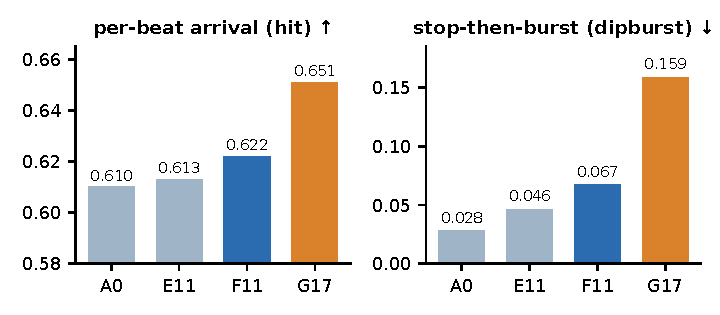
\includegraphics[width=0.6\linewidth]{figures/metric_gaming.pdf}
  \caption{\textbf{A gamed metric} (nine whole songs, 3D). G17 wins on per-beat arrival but more than doubles abrupt stop-then-burst events; viewers preferred F11.}
  \label{fig:gaming}
\end{figure}

\subsection{Diagnostics and negative results}
\label{sec:ablation}

The following measurements shaped the design and are, in our view, as informative as the positive results.
\begin{itemize}
  \item \textbf{Pose statistics were not the gap.} Before the timing work, generated dances already matched ground truth on knee flexion ($0.908$ vs $0.900$), hands above shoulders ($42.6\%$ vs $45.7\%$), pose change between beats ($0.429$ vs $0.424$) and move-change rate ($0.526$ vs $0.445$). Yet ground truth locked to its own song's beat grid ($+0.034$ against other songs, 14/19, $p{=}0.03$) and no generated variant did.
  \item \textbf{Retrieval was not the bottleneck.} Substituting randomly chosen ground-truth bars kept most of the beat lock.
  \item \textbf{Completion helps, and music guidance inside it does nothing.} Widening the inpainted seam from $0$ to $16$ frames reduced the largest single-frame yaw jump from $48.5^\circ$ to $31.9^\circ$. Changing the music guidance weight from $1.0$ to $3.0$ changed joint positions by at most $0.18$\,mm; the completion model acts as a smoothing prior, which is why timing must be decided before it.
  \item \textbf{Stretching and seam windows.} An earlier recipe blended $\pm 8$ frames at every seam and overwrote the arrival of a move on strong beats (13.7\,cm on average); moving the transition after the bar line reduced this to 2.9\,cm and seam jerk from $1.045$ to $0.631$ (10/10 clips, $p{=}0.002$).
  \item \textbf{Premises that did not hold.} Real dancers do not return to a movement where the melody repeats (Spearman $0.018$ vs null $0.007$, $p{=}0.63$, although a planted-copy test detected returns with $p{=}10^{-16}$), and denser music does not produce denser steps ($+0.014$ vs shuffled $+0.028$). Picking the largest, most extended movements (``prefer full'') raised extension but was rejected by the operator, and its render hit the beat worse.
  \item \textbf{The planner vocabulary matters more than the planner.} Music identifies the recording a bar comes from very well but predicts discovery labels below the majority floor; the planner's label distribution is broad (entropy $2.93$ of $3$ bits), and hand usage varies little between labels, so the lever is the choice \emph{within} a label---the motivation for the label-to-motion criteria.
\end{itemize}

% =====================================================================
\section{Limitations}
\label{sec:limitations}

\begin{itemize}
  \item \textbf{One creator.} The corpus contains performances by a single dancer, so the vocabulary, library and all numbers reflect one style. Generalization to other dancers, genres and group dances is untested.
  \item \textbf{Small, imperfect held-out set.} The test set has 20 clips. The fingerprint-based split missed at least one same-recording pair across test and train and one across validation and train. Several variants were compared, and the planner seed chosen, on the same test and validation clips, so the reported comparisons are not a clean held-out estimate. Some full-song renders include a song that also appears in training.
  \item \textbf{No standard benchmark comparison.} We do not report results on AIST++ or FineDance, nor against published generators under a common protocol; our metrics are designed for in-the-wild data and for diagnosing timing, not for leaderboard comparison.
  \item \textbf{Metrics are partly selected on.} Step lock and energy following select candidates on quantities close to the metrics that evaluate them. We mitigate this with controls, a second plan, full songs, rendered-video measurements and human review, but the effect sizes on the targeted metrics should be read with that in mind.
  \item \textbf{Human evaluation by one reviewer.} Visual verdicts come from the project's operator rather than a user study. K13 has not yet received such a verdict.
\end{itemize}

% =====================================================================
\section{Conclusion}

BarLine Dance treats the musical bar as the unit of choreography and moves the decision of \emph{when} a movement happens into the stage that chooses real recordings for each bar.
Choosing candidates by where their steps land on the song's beat grid, by whether the same dancer can continue across the bar line, and by how their energy matches the song's loudness produced dances whose timing is specific to the song they dance to---measured against explicit null controls and confirmed on rendered video.
Our experience also suggests a methodological point for dance generation: metrics that are not validated against controls, or that can be satisfied by an unnatural behavior, will eventually select the wrong model, and watching the dance remains indispensable.

\bibliographystyle{plainnat}
\bibliography{refs}

\end{document}
